\chapter{Implementation}

This chapter covers the detailed implementation of all components needed for integrating Apache Ranger as an access control system for OpenMetadata. We also present engineering problems that arose during the implementation process and their solutions.

\section{Relocating the OpenMetadata Authorizer interface and related classes}

We begin by investigating the current Authorizer interface used by OpenMetadata, shown in Listing \ref{listing:original_authorizer}. The functions \mintinline{java}{listPermissions} and \mintinline{java}{getPermission} are used to query the operations a user is allowed to apply on all resource types, all resources under a specific resource type or a fully-qualified resource. The \mintinline{java}{authorize} function handles access control decisions, yielding successfully when access is authorised and throwing an \mintinline{java}{AuthorizerException} when it is not. The \mintinline{java}{authorizeAdmin} directive verifies that a user is an administrator of the system, throwing an exception otherwise. The final procedure, \mintinline{java}{decryptSecret}, is the process of being deprecated. 

The interface, along with all classes and other interfaces used in its definition, is part of the \mintinline{text}{org.open-metadata:openmetadata-serivce} submodule and is tightly bound to OpenMetadata's API service implementation. This is an issue, as the Apache Ranger authoriser implementation needs to be isolated in a separate submodule that does not depend on \mintinline{java}{openmetadata-service}. The solution proposed here is to relocate the \mintinline{java}{Authorizer} interface, with related classes and interfaces, to a new submodule \mintinline{text}{org.open-metadata:openmetadata-authorization}; thus, the API service implementation submodule and Apache Ranger authoriser submodule may then depend on it.

We define that \mintinline{text}{org.open-metadata:openmetadata-authorization} submodule to depend on the \mintinline{text}{org.open-metadata:openmetadata-spec} module, providing entity definitions, and to contain four interfaces under the \mintinline{java}{org.openmetadata.security} package: \mintinline{java}{Authorizer}, \mintinline{java}{OperationContextInterface}, \mintinline{java}{ResourceContextInterface}, \mintinline{java}{SecurityContextInterface} and the \mintinline{java}{AuthorizationException} class. The \mintinline{java}{Authorizer} interface is updated to use the new interfaces.

\begin{listing}

\begin{minted}[breaklines,
    linenos,
    fontsize=\footnotesize,
    frame=single,
]{java}
public interface Authorizer {
    void init(OpenMetadataApplicationConfig openMetadataApplicationConfig, Jdbi jdbi);

    List<ResourcePermission> listPermissions(SecurityContext securityContext, String user);

    ResourcePermission getPermission(SecurityContext securityContext, String user, String resource);

    ResourcePermission getPermission(
        SecurityContext securityContext, String user, ResourceContextInterface resourceContext);

    void authorize(
        SecurityContext securityContext, OperationContext operationContext, ResourceContextInterface resourceContext)
        throws IOException;

    void authorizeAdmin(SecurityContext securityContext);

    boolean decryptSecret(SecurityContext securityContext);
}
\end{minted}

\caption{Original \mintinline{java}{org.openmetadata.service.security.Authorizer} interface in the OpenMetadata source code.}
\label{listing:original_authorizer}

\end{listing}

\subsection{Initialisation}

The \mintinline{java}{OpenMetadataApplicationConfig} and \mintinline{java}{Jdbi} classes are part of the \mintinline[breaklines, breakafter=.:]{java}{org.open-metadata:openmetadata-serivce} module can not be used in the authorisation interface.

OpenMetadata handles the initialisation of resources in the \mintinline{java}{OpenMetadataApplication} class. The authoriser instance is created based on the \mintinline{text}{authorizerConfiguration.className} property provided by the application configuration. The following expression handles class loading and instance creation, the configuration properties being passed later to the \mintinline{java}{init} function.

\begin{minted}[breaklines, breakbefore=.]{java}
    this.authorizer = Class.forName(authorizerConf.getClassName()).asSubclass(Authorizer.class).getConstructor().newInstance();
\end{minted}

The initialisation sequence is updated to use the class constructor that takes a single argument, an instance of \mintinline{java}{AuthorizerConfiguration}, and the \mintinline{java}{init} function is modified to take no arguments.

\begin{minted}[breaklines, breakbefore=.]{java}
    this.authorizer = Class.forName(authorizerConf.getClassName()).asSubclass(Authorizer.class).getConstructor(AuthorizerConfiguration.class).newInstance(authorizerConf);
\end{minted}

The provided authoriser implementations, \mintinline{java}{DefaultAuthorizer} and \mintinline{java}{NoopAuthorizer}, are updated to follow the revised structure. Listing \ref{listing:new_authorizer} provides the final layout of the authorisation interface that the Apache Ranger authoriser will implement.

\begin{listing}

\begin{minted}[breaklines,
    linenos,
    fontsize=\footnotesize,
    frame=single,
]{java}
public interface Authorizer {
    default void init() {}

    List<ResourcePermission> listPermissions(SecurityContextInterface securityContext, String user);

    ResourcePermission getPermission(SecurityContextInterface securityContext, String user, String resource);

    ResourcePermission getPermission(
        SecurityContextInterface securityContext, String user, ResourceContextInterface resourceContext);

    void authorize(
        SecurityContextInterface securityContext,
        OperationContextInterface operationContext,
        ResourceContextInterface resourceContext)
        throws IOException;

    void authorizeAdmin(SecurityContextInterface securityContext);

    boolean decryptSecret(SecurityContextInterface securityContext);
}
\end{minted}

\caption{Updated \mintinline{java}{org.openmetadata.service.Authorizer} interface in the OpenMetadata source code.}
\label{listing:new_authorizer}

\end{listing}

\section{Using Apache Ranger libraries for authorisation}

This section details the initialisation and utilisation of Apache Ranger libraries for access control policy evaluation through the \mintinline{java}{RangerBasePlugin} class. It also touches on using the Hadoop user group information utility to retrieve users' group membership data for a centralised Active Directory database.

\subsection{Initialisation of the Ranger Plugin}

The Ranger base plugin loads its configuration from XML files structured as lists of key and value string pairs. This behaviour is handled by the \mintinline{java}{RangerPluginConfig} class that extends the commonly used Hadoop class \mintinline{java}{Configuration}.

Apache Ranger's configuration loading utility expects properties to be provided in three files, \mintinline{text}{ranger-<serviceType>-audit.xml}, \mintinline{text}{ranger-<serviceType>-security.xml} and\\ \mintinline{text}{ranger-<serviceType>-policymgr-ssl.xml} (where \mintinline{text}{<serviceType>} is a placeholder for the type of the service that the plugin is being initialised for, in this case taking the value \mintinline{text}{openmetadata}), which it will attempt to read from the current directory. We extend this functionality by allowing administrators to specify alternative locations for these files in OpenMetadata's configuration. The Hadoop utility for querying user group information is initialised similarly. Sample configuration files are in the OpenMetadata source code under the \mintinline{text}{ranger/openmetadata-authorization-ranger/conf} folder.

\section{\label{sec:utilising_the_ranger_plugin} Utilising the Ranger Plugin}

The Ranger plugin evaluates access requests using the function \mintinline{java}{isAccessAllowed}, which takes a single argument, an instance of the \mintinline{java}{RangerAccessRequest} class which wraps identification of the user requesting access (consisting of the user's unique name and the groups and roles it is a member of), a description of the resource being accessed, and the operation applied to the resource. 

User identification is handled by the mintinline{java}{RangerHadoopUserGroupsRolesProvider} class. Resolving the need data begins with the \mintinline{java}{SecurityContextInterface}, which supplies the user's name. The Ranger Authorizer uses the Hadoop User Group Information utility to get the user's groups.

\begin{minted}[breaklines, breakbefore=.]{java}
Set<String> groups = UserGroupInformation.createRemoteUser(internalName).getGroupNames();
\end{minted}

The Ranger Plugin is then used to retrieve the appropriate roles based on the user's name and the groups.

\begin{minted}[breaklines, breakbefore=.]{java}
Set<String> roles = rangerPlugin.getRolesFromUserAndGroups(user, groups);
\end{minted}

The Ranger Plugin handles references to resources as a mapping between string keys, representing the resource type, and generic objects, representing the value of the resource type, through the \mintinline{java}{RangerAccessResourceImpl} class. The generic objects used for resource values are commonly strings or collections of strings. The \mintinline{java}{RangerOpenmetadataAccessResource} class extends \mintinline{java}{RangerAccessResourceImpl}, implementing the mapping of OpenMetadata entities to key-values pairs recognised by the Ranger Plugin. The class handles setting values for entities with parents by reflectively invoking methods that take certain entity types as arguments, as depicted in Listing \ref{listing:ranger_openmetadta_access_resource}.

Since these are recursive types, Tag and Glossary Term entities require specialised resource-value mapping. A Tag object does not provide a reference to its Tag Category or parent Tag; thus, we build the resource path of a Tag from its fully quantified name. OpenMetadata defines a language for the fully qualified names of entities, a dot-separated list of strings which may be in quotes if containing special characters, using ANTLR; fully qualified names are split into their components by parsers generated by ANTLR. The Tag Category and ancestor Tags of a Tag entity can thus be derived from the elements of its fully qualified name. A Glossary Term entity contains references to its Glossary and parent Term, but to retrieve the parent of the parent Glossary Term a database read is required; we avoid this inefficiency but adopting the same approach as with Tag entities. For both Tags and Terms, the ancestors' names are joined with the forward-slash symbol (/) to create path-like strings recognised by the Ranger Plugin.

\begin{listing}

\begin{minted}[breaklines,
    linenos,
    fontsize=\footnotesize,
    frame=single,
]{java}
public class RangerOpenmetadataAccessResource extends RangerAccessResourceImpl {
    public RangerOpenmetadataAccessResource(ResourceContextInterface resourceContextInterface) {
        ...
        EntityInterface entity = resourceContextInterface.getEntity();
        try {
            Method method = this.getClass().getDeclaredMethod("setSubValues", entity.getClass());
            method.invoke(this, entity);
        } 
        ...
    }
    
    private void setSubValues(Table table) {
        setValue(table.getService(), DatabaseService.class);
        setValue(table.getDatabase(), Database.class);
        setValue(table.getDatabaseSchema(), DatabaseSchema.class);
    }
    
    ...

    private void setValue(EntityReference entityReference, Class<? extends EntityInterface> clazz) {
        if (entityReference == null) {
            setValue(formatOpenMetadataClassNameToRangerResource(clazz), "*");
        } else {
            setValue(entityReference);
            }
    }

    private void setValue(EntityReference entityReference) {
        setValue(getRangerResourceName(entityReference), entityReference.getName());
    }
}
\end{minted}

\caption{Snippet of the \mintinline{java}{RangerOpenmetadataAccessResource}, using reflection to set Ranger Access Resource values from OpenMetadata entities.}

\label{listing:ranger_openmetadta_access_resource}

\end{listing}

The access type is passed to the Ranger Plugin as a string, retrieved from the \mintinline[breaklines, breakbefore=CI]{java}{OperationContextInterface}. As this interface provides a list of operations, each is checked independently.

Listing \ref{listing:ranger_authorizer_impl_authorize} supplies the body of the \mintinline{java}{authorise} function provided by the Ranger Authorizer implementation of the OpenMetadata \mintinline{java}{Authorizer} interface. The procedure uses the \mintinline{java}{RangerOpenmetadataAccessRequest} class, which extends the provided request class \mintinline[breaklines, breakbefore=ARI]{java}{RangerAccessRequestImpl}, adding convenience constructors. The \mintinline{java}{isAccessAllowed} procedure of the Ranger Plugin returns a \mintinline{java}{RangerAccessResult} object, which contains the final allowed or denied decision along with meta information of the policy evaluations.

\begin{listing}

\begin{minted}[breaklines,
    linenos,
    fontsize=\footnotesize,
    frame=single,
]{java}
public void authorise (
        SecurityContextInterface securityContext,
        OperationContextInterface operationContext,
        ResourceContextInterface resourceContext)
        throws IOException {
    RangerUserGroupsRoles ugr = groupsRolesProvider.getUserGroupsRoles(securityContext);
    RangerAccessResource accessResource = new RangerOpenmetadataAccessResource(resourceContext);
    for (MetadataOperation operation : operationContext.getOperations()) {
        RangerAccessRequest req = new RangerOpenmetadataAccessRequest(accessResource, operation, ugr);
        RangerAccessResult result = rangerPlugin.isAccessAllowed(req);
        if (result != null && !result.getIsAllowed()) {
            throw new AuthorizationException(String.format("[RangerAccessRequest=%s] Permission denied by Ranger: %s", req, result));
        }
    }
}
\end{minted}

\caption{Snippet of \mintinline{java}{RangerAuthorizerImpl}, displaying the implementation of the authorisation check.}
\label{listing:ranger_authorizer_impl_authorize}
    
\end{listing}

\subsection{Listing user permissions for resources}

The Ranger Plugin enables queries of access control rules (commonly abbreviated to ACLs) with the procedure \mintinline{java}{getResourceACLs}, which accepts a single argument, a \mintinline[breaklines, breakbefore=AR]{java}{RangerAccessRequest} object. Creating an access request is the same as detailed above. An additional case appears when querying permissions for all resources of a type, which is handled by mapping, in the \mintinline{java}{RangerAccessResourceImpl}, the resource type and its ancestor to wildcards (the asterisk symbol).

The \mintinline{java}{getResourceACLs} function returns a \mintinline{java}{RangerResourceACLs} object containing three maps of the type \mintinline{java}{Map<String, Map<String, AccessResult>>}, one for each of user, group and role access control rules. Keys of the outer map represent the name of a user, group or role, respectively, while keys of the inner map represent access type, and values of the inner map represent an access result, which can be allowed, denied or undetermined. This response is not aggregated, as it will contain results for all users, groups and roles present in policies that match the resource queried and outcomes for all access types, not only those applicable to the resource type used in the request. Results are consolidated by the \mintinline{java}{RangerPermissionsProvider} class, filtering groups and roles the user is not part of and access types which do not correspond to the resource type in question, and combines the remaining results. An access type is considered permitted if any of the user's groups for roles allow it or if the user is specifically allowed that access type.

\section{Additional changes to OpenMetadata}

This section details changes to OpenMetadata's metadata service and user interface to empower better compatibility with the Ranger authoriser's more precise access control mechanism. When considering these changes, supporting complete backward compatibility and maintaining the same behaviour for the included authoriser is critical.

\subsection{Listing of entities}

OpenMetadata's included authorisation system does not distinguish between entities with the same resource type; thus, listing entities of a kind (e.g., tables) is authorised by checking that the principal user is allowed to perform the ViewAll action on all resources of that type. This approach does not operate well with the more precise access control imposed by the Ranger authoriser, where a user may be allowed to view a subset of tables but not all.

The listing of entities paginates results, returning two pointers to the start and end of the list of results, which can be used by future requests to fetch the next or previous page of entities. As the access control evaluation is done inside the metadata service, it cannot be known if the user is allowed to view a resource before fetching it from the database; at the same time, it is ideal for reducing the number of entities unnecessarily retrieved from storage. The solution proposed fetches singular entities, checks access permission for the user on that resource and adds it to the page or discards it accordingly until the page is filled. This approach avoids the issue of retrieving too many entities so that the page is completed before all can be evaluated, thus wasting resources; it is a trade-off between the cost of a round-trip to the database and the cost of transporting and deserialising more data. 

\subsection{Masking results on the Search page}

OpenMetadata maintains a copy of the metadata in Elasticsearch, which is used for fast searches, input autocompletion and aggregations. Searching through entities is available with two API endpoints  \mintinline{text}{/api/v1/search/query} and \mintinline{text}{/api/v1/search/suggest}. These endpoints only enable the reading of some metadata entities but bypass the access control mechanisms; thus, metadata that the user is not privileged to view can appear in the search results. This is a known security issue of the platform, with plans to fix it in future versions. It is also a complex issue to resolve since the access control system may add too much overhead to the search functionality, diminishing one of its main primary purposes, fast resource lookup; additionally, since filtering of results from the search engine needs to be done by the metadata service, the values of total results, hit scoring and aggregations would be skewed. For these reasons, the issue of access control mechanism for search results in OpenMetadata is beyond the scope of this report.

We provide a mechanism for signalling to the users using the Search page in OpenMetadata's user interface that they are not privileged to view some of the entities presented. Recall Figure \ref{fig:openmetadata_sample_data_explore}, showing the Search page and the right-hand side panel, which appears when the user clicks on one of the search results. If the user is not allowed to view the entity (table in this case), the panel will not show any data, instead displaying a suitable message, as illustrated in Figure \ref{fig:openmetadata_sample_data_explore_denied}. The feature is implemented as part of the UI, calling the \mintinline{java}{/api/v1/permissions/{resource}/{id}} API endpoint to list the permissions of the current user on the given resource.

It is essential to highlight that this change does not provide any improvements to the security of the system, as data is still available programmatically - it is only an improvement to the user experience.

\begin{figure}
    \centering
    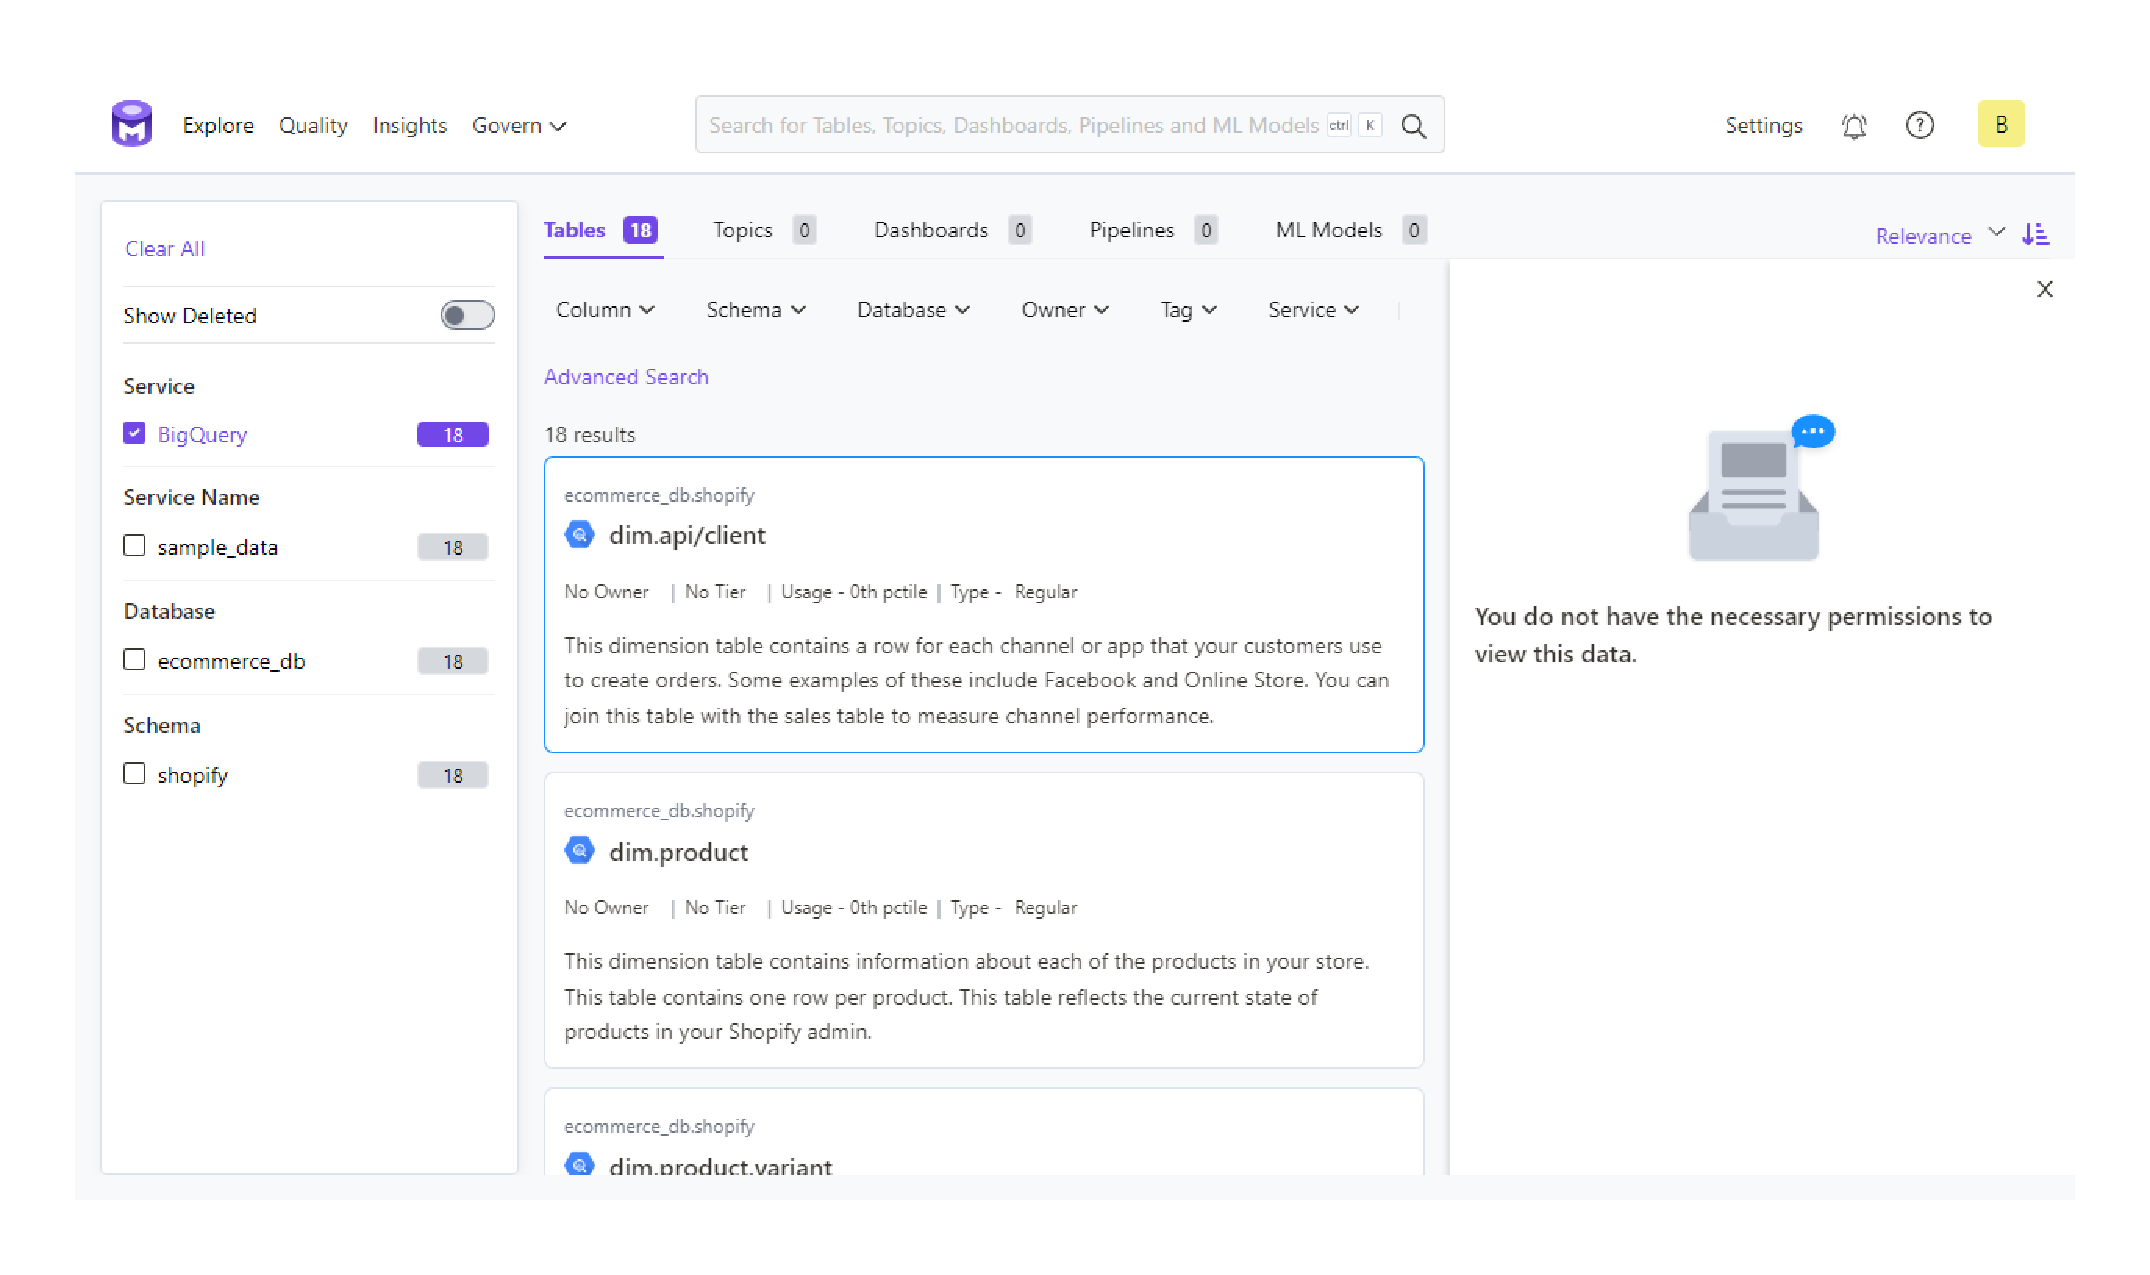
\includegraphics[width=\textwidth]{chapters/implementation/figures/openmetadata_sample_data_explore_denied.pdf}
    \caption{Screenshot of OpenMetadata's Search page, showing the "Access Denied" side panel.}
    \label{fig:openmetadata_sample_data_explore_denied}
\end{figure}

% \subsection{Build artefacts}

% The build artefacts generated by the OpenMetadata project are a tarball and an RPM file. All compiled Java classes and their dependencies are added to the \mintinline{text}{libs} folder so these can be loaded into the classpath of the Java process. The Ranger authoriser handles loading its classes and dependencies using the shim class.